\documentclass[12pt, ]{scrartcl}
\usepackage[style=alphabetic]{biblatex}
\usepackage{graphicx}
\usepackage{float}
\graphicspath{{./graphics}}
\addbibresource{bibliography.bib}
\usepackage{multicol}
\usepackage{setspace}
\usepackage[hidelinks]{hyperref}
\usepackage[capitalise]{cleveref}
\usepackage{titleref}
%opening
\title{Improvement of the Bayesian generalization model in order to handle negative examples and discontinuous hypotheses}

\begin{document}
\def\isblind{1}
\def\doublecol{1}
\def\doublespace{0}
\if\isblind0
    \author{Jason Cramer, Maximilian Dierschke, Nils Engleder}\fi
\if \isblind1
    \author{}\fi

\maketitle
\if \doublespace1
	\doublespacing \fi
	
\if \doublecol1
\begin{multicols}{2}
	\fi
\section{Background}
The problem our project is focusing on is Shepard's ideal generalization problem. The generalization problem focuses on how humans build hypothesis spaces for a given consequence after observing stimuli.
In the paper "Generalization, similarity, and bayesian inference", they discuss how using a model of bayesian inference, we can predict the probability of given stimuli being included within the consequential region \cite{Tenenbaum}.
The model uses the equation $p(y \in C \mid x) = \sum\limits_{h:y\in h} p(h | x)$ where $h$ is a hypothesis from the hypothesis space ${\cal H}$ and $p(h | x)$ is the posterior probability of  the hypothesis after observing x.
We extend this model to investigate how including negative examples within the x vector(x is the observed stimuli) affect how the model limits hypotheses. Furthermore, do we try to compute multiple consequential regions given positive positive examples. We also plan to explore how different distributions and models compare to the original model for generalization.
\section{Question}
To generalize the model by Tenenbaum et al, we want to find a way, how it can be improved, so that it can handle negative examples and discontinuous hypotheses.

\section{Negative examples in the baseline model}
The baseline model (Figure \ref{fig:baseline}), which was introduced by Tenenbaum et al. is by itself not capable of handling negative examples. 

A naive approach to incorporate negative examples, is to fit two models, where one represents the positive and one represents the negative examples. To combine both aspects, the predicted probability from the model for the negative examples is then subtracted from the prediction for the positive examples. 
Since the model calculated probabilities, it needs to be ensured, that the sum does not go below zero and therefore the outcome needs to be rectified.

\begin{figure}[H]
	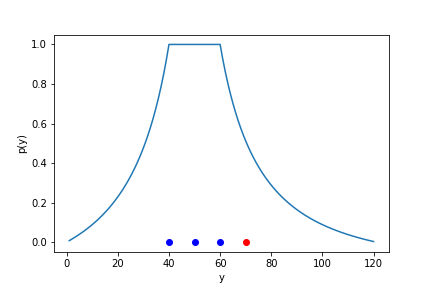
\includegraphics[scale=0.5]{graphics/baseline.png}
	\caption{Baseline Model fitted on positive samples [40, 50, 60] (blue) does not incorporate the negative example [70](red) }
	\label{fig:baseline}
\end{figure}

With the same data points as before, a shark fin like function is the result. 
As expected, has the negative example a probability of 0. As it can be seen in (Figure \ref{fig:add1}) is the prediction for positive examples less than 1. \\
This function therefore is able to capture some of the features that would be expected to be seen from a human in this example, but not quite what is expected.
\begin{figure}[H]
	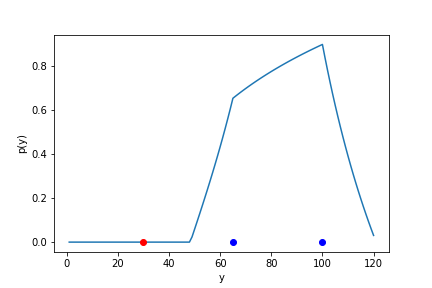
\includegraphics[scale=0.5]{graphics/addition_model}
	\caption{Addition Model fitted on positive samples [40, 50, 60] (blue) and negative samples [70] (red)}
	\label{fig:add1}
\end{figure}

Next, a negative example is put in the middle between two positive examples.
When the addition model is then used on that data, it predicts the positive data points to have the highest probability and it tapers off towards the negative example (Figure \ref{fig:add2}). 
Unfortunately, it does predict less than 100\%, for positive examples, which would be expected. 
Although this model is so simple, it captures some of the underlying principles well enough. 

\begin{figure}[H]
	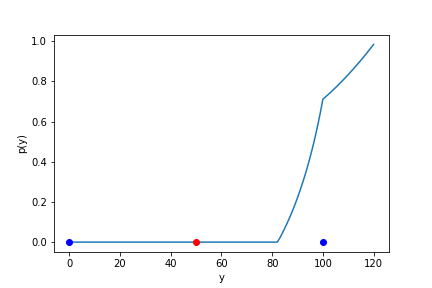
\includegraphics[scale=0.5]{graphics/addition_model_multiple_regions}
	\caption{Addition Model fitted on positive samples [1, 100] (blue) and negative samples [50] (red)}
	\label{fig:add2}
\end{figure}
	 
	
\section{Limiting positive regions using negative examples}\label{sec:elim}
%(3) Evaluate how the model could be altered so that negative examples can be incorporated to limit cluster intervals assuming a continuous consequential region
In order to get a more accurate representation of the problem at hand, the negative examples can be used in a different way.
A typical use case for negative samples under the assumption of a single positive region is limiting that region. 
This follows from the general behavior of fitting assumptions to reference points.
We would typically refer to the underlying thought process as one of elimination, since the knowledge of counterexamples is used to discard hypotheses.
Thus we shall call the corresponding model the elimination model.
Since our baseline model takes all possible hypotheses into consideration, the process of integrating counterexamples is relatively straightforward: We remove all those hypotheses from consideration which are contradicted by our negative examples.
To this end, we modify the likelihood calculation to return zero for all hypotheses which would incorporate a known negative example, therefore removing those hypotheses from consideration.
This results in the posterior probabilities for all values on the far side of a negative sample (from the perspective of a positive sample) being zeroed out, while retaining the exponential falloff behavior of the base model.

\begin{figure}[H]
	\centering
	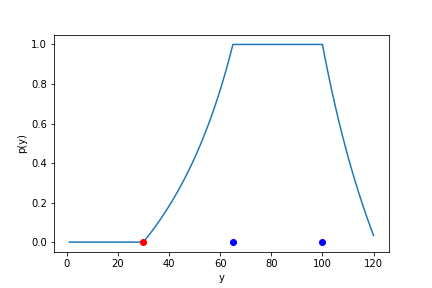
\includegraphics[scale=0.5]{graphics/elimination_model}
	\caption{Elimination Model fitted on positive samples [40, 50, 60] (blue) and negative sample [70] (red)}
	\label{fig:elim}
\end{figure}

As can be seen in the plot of our example data (\cref{fig:elim}), the predictions generated by this approach correctly match the 0\% probability we would expect to see for known negative samples.
Otherwise, the general shape of the baseline curve is retained.
This corresponds to the assumption of additional information on the limits of the maximal positive region having no influence on the expected prediction falloff.
Intuition suggests this is a reasonable assumption to make, since there is no apparent difference between the limits of the consequential region and limits of any maximal positive region (limited by negative samples) within it.

\begin{figure}[H]
	\centering
	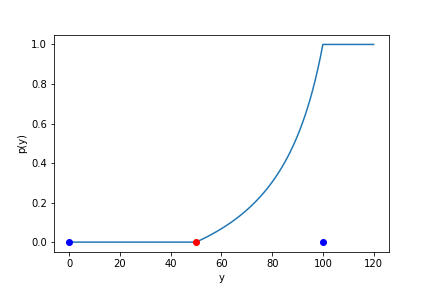
\includegraphics[scale=0.5]{graphics/elimination_model_multiple_regions.png}
	\caption{Elimination Model fitted on positive samples [1, 100] (blue) and negative samples [50] (red)}
	\label{fig:elim1r}
\end{figure}

\section{Separating positive regions by negative examples}\label{sec:elimsum}
%(4) Evaluate how the model could be altered so that negative examples can be incorporated to limit cluster intervals assuming a discontinuous consequential region
The Elimination Model (\cref{sec:elim}) fails on sample data which corresponds to disjoint positive regions with interspersed negative samples (\cref{fig:elim1r}) due to eliminating all probable hypotheses from its calculated space of continuous hypotheses.
In order to address this shortcoming, we can pre-process the sample data and split every continuous section of positive samples into its own instance of the elimination model.
By slicing the list of positive examples using the list of negative examples, we get non-overlapping segments limited either by the bounds of the consequential region or a negative sample.
In either case the elimination model will zero out all posterior probabilities beyond this boundary, generating independent peaks for each continuous positive region
Thanks to the guaranteed lack of overlap between slices, prediction data can be recombined by summing the posterior probability vectors of all model instances to create the final prediction vector for the entire consequential region (\cref{fig:elim_sum}). 
\begin{figure}[H]
	\centering
	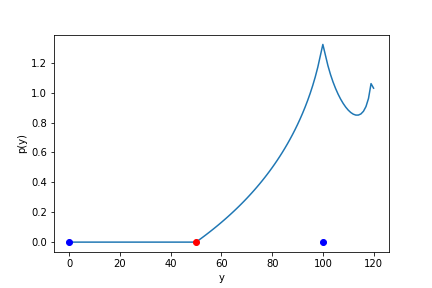
\includegraphics[scale=0.5]{graphics/elimination_sum_model.png}
	\caption{Elimination-Sum Model fitted on positive samples [1, 100] (blue) and negative samples [50] (red)}
	\label{fig:elim_sum}
\end{figure}
Note that this model relies on negative samples to identify and limit disjoint or partial positive regions. As this model performs identical to the Elimination Model (\cref{sec:elim}) for inputs it can handle and additionally produces sensible predictions for sample data that would result in computation errors, it can be considered an universally superior alternative.

\section{Multiple Discontinuous Regions Model}
To explore how people predict the consequential region when using a model with multiple discontinuous regions, we will use
a modification of the original model, which allows for multiple discontinuous regions.
\begin{figure}[H]
	\centering
	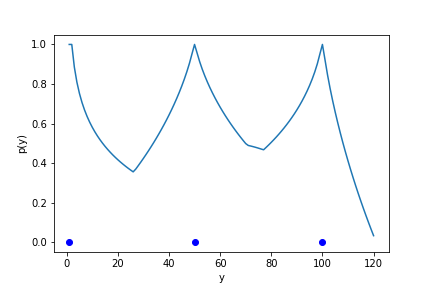
\includegraphics[scale=0.5]{graphics/mprm_model}
	\caption{Multiple Discontinuous Regions Model fitted on samples [1, 100] with 2 expected (disjoint) regions}
	\label{fig:mprm}
\end{figure}
In the case that there are multiple clusters of data points, we expect, that humans would  give higher likelihoods for the clustered regions than their surrounding areas. 
This behavior is shown well by the function, which can be seen in \cref{fig:mprm}. The resulting function shows the expected characteristics, but is not as smooth as it would be expected.
It works by splitting the stimuli into n-regions and then calculating the posterior probability for each region.
This model is fitted to only positive examples, and works by taking $\max{p_i(observation)}$, 


In the classroom example ( with a negligible statistical significance) the test subject did not predict, what we were hoping for. Instead, the probability was picked close to one for the whole arrange between the positive examples.  
This is due to the binning process which works in the following way:
\begin{enumerate}
	\item Calculate the splitting distance $\textbf{s} = \frac{\sum\limits_{x_i \in X} x_i}{number of regions}$
 	\item For each samples $x_i$ calculate the bin number $i$ as $\textbf{i} = \left\lfloor \frac{x_i}{s} \right\rfloor$
\end{enumerate}
This process works well for spacious data, however, fails for higly clustered data. 
\section{Conclusion}

We were able to design models that were able to predict:
\begin{itemize}
	\item Continuous regions with negative examples
	\item Discontinuous regions with negative examples
	\item Discontinuous regions with only positive examples 
\end{itemize}

We created the models based on our intuition of how we think people think. Therefore an experiment to validate (or invalidate) our models would be a good future work.


\printbibliography

\if \doublecol1
\end{multicols}
\fi

\newpage
\section*{Group member collaboration}
All participants of the group project collaborated on the solutions together and contributed equally to the project outcome. 

\end{document}
